\subsection{Task Design}
After exploring and analyzing many gamified systems and the effect of various game elements towards user engagement and motivation, Sailer et al. \cite{45} argues that gamification is not effective per se, but specific game design elements have specific psychological effects. Thus, it is important that gamification is not done just by incorporating a scoring system with some levels to advance and a leaderboard to see your progress. It takes more than that to design a game that attracts and retains a player base. 

Chamberlain et al. \cite{43} emphasizes that it is the design of the individual tasks in a gameplay that determine how successful the player can contribute data whilst playing. Furthermore, Sailer et al. \cite{45} communicates the importance of game elements being recognized by the player in the gamified environment. Delivering the treatment to the player or to a participant in the game is not enough unless the designer of the game makes sure that the treatment is also received by them. Failing to design treatments or game elements that are genuinely recognized by the players, results in loss of statistical power and risk to underestimate their effectiveness \cite{45}. In order to adhere to the aforementioned design constraints, significant work effort was placed in designing a task that contributes to generating annotation data of good quality. 


A game-round starts by the player selecting a specific category to play or letting the game choose a category in a random fashion for the player. Everything in the game is designed in a way that the player only has to use the keyboard for completing almost every action. The player is then presented with the typing screen where a combination of hidden characters have to be revealed by typing as fast as possible. Figure \ref{fig:game-typingscreen} illustrates the typing screen. A speed radar is placed right underneath the typing text box which displays the current speed of typing measured as the amount of words typed per minute while the player is revealing the hidden characters. This element can be considered a strong motivator to keep the player focused on typing fast. After having revealed the word, the upcoming challenges/questions all revolve around the text that has been typed during the typing phase. The players are already familiar with this concept since a similar task was already performed during the onboarding phase. Bonus questions are immediately presented to the user after completing the revealing stage (we talk more about the importance of bonus questions towards the overall design in a later subsection). The content of the bonus questions is created by using the text that was typed in the previous stage. Similarly, the most important part of the game that contributes to the original task of disambiguating entities is the quiz stage of the game. The quiz interface provides contextual clues extracted from our original framework and lists all the potentially candidates (quiz options) from which the player has to choose. 

\begin{figure}[]
  \centering
  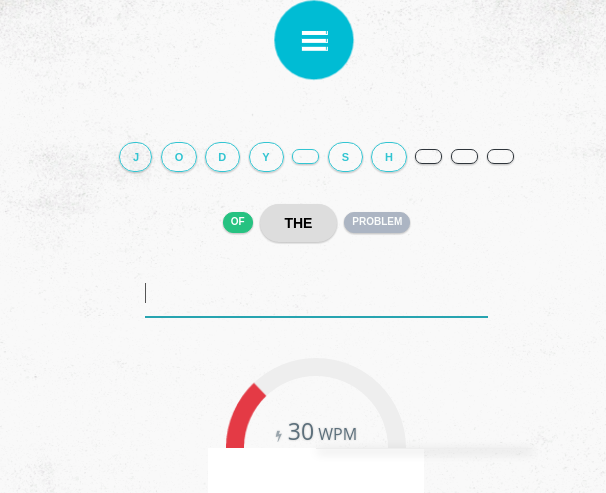
\includegraphics[width=.6\linewidth]{figures/experiment2/gameplay1.png}
  \caption{The typing screen and the speedometer calculating the typing speed of the player}
  \label{fig:game-typingscreen}
\end{figure}

We strongly emphasize the fact that all the game elements presented so far are focused and contribute to the ultimate goal, which is annotating the entity with the right candidate. The text which the player types during the typing stage, the content of the bonus questions and the contextual clues all represent carefully carved information that contribute in helping the player choose the right candidate. We make sure that the typing text\footnote{During the fast-typing stage, players are presented with different words that appear on the screen one after another. These words are part of a complete paragraph that is taken from the document where the target entity is part of.} as a game element is recognized and takes the attention of the player because if players are able to remember the text they typed, they can get points from correctly answering the bonus questions and also be confident on the candidate option they select. An example of a bonus question is presented in Figure \ref{fig:game-bonusqeustion} while the quiz interface of the game is illustrated in Figure \ref{fig:game-quiz}. 

\begin{figure}[]
    \centering
    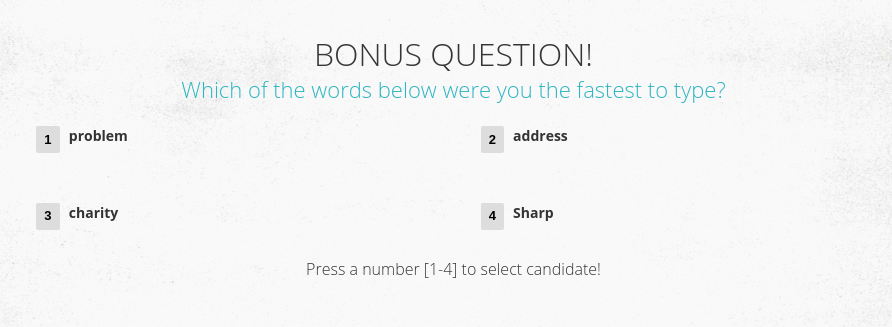
\includegraphics[width=.8\linewidth]{figures/experiment2/bonusquestion.png}
    \caption{An example of a bonus question}
    \label{fig:game-bonusqeustion}
\end{figure}

\begin{figure}[]
    \centering
    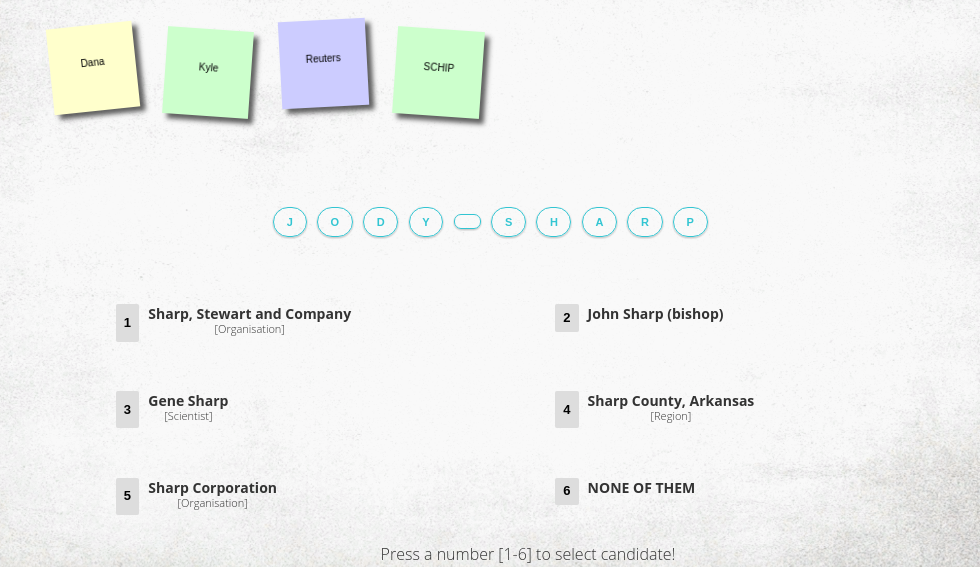
\includegraphics[width=.6\linewidth]{figures/experiment2/game-quiz.png}
    \caption{Interface of the game quiz - a gamified version for the named entity disambiguation task}
    \label{fig:game-quiz}
\end{figure}

%Skillset required/improved in the game
Schell \cite{51} (page 214) emphasizes the importance of the skill and chance mechanisms in games. A good game should balance between skill and chance during the gameplay. We believe that we have reached a satisfactory balance between these two factors by equalizing the factor of chance and skill required. The factor of luck is represented by bonus questions which are extracted from the typing text and are genuinely hard to answer since a memorization of everything typed is required. On the other hand, the factor of skills is represented by the quiz element of the gameplay. Correctly answering the quiz requires certain skill-sets from the player in order to maximize their profit point-wise. Except requiring skills from the players, the game should also contribute in allowing the players to master and perfection these skills. In general, by playing Fastype, a player will improve the following skills:

\begin{itemize}
    \item Typing skills
    \item Concentration in time pressure 
    \item Memory training and pattern recognition
    \item Knowledge in different categories (politics, music, entertainment, health etc)
\end{itemize}

Improving these skills is one of the goals that players will attempt to achieve. After having observed the players during their gamplay when conducting the second experiment we are aware that the goals of the game are concrete, achievable and rewarding at the same time. Having all these three elements characterizing the goals of the game is crucial to keeping players engaged and motivated \cite{51}. 

Reviewed literature suggests a number of criteria for evaluating enjoyment during gameplay. Some of the criteria which apply to task design and which also relate with SDT in terms of their importance towards increasing intrinsic motivation include: Feedback and Immersion \cite{41}. Constant feedback is given to the player for every performed action when interacting with Fastype. Immersion in our case refers to a short and arcade style of the gameplay which make the player experience a deep and yet effortless involvement in the game \cite{41}. A game round in Fastype lasts 4-5 minutes on average with the player being exposed to different challenging tasks. This results in an effortless and deep involvement in the game for a short period of time. Additionally, the game elements and the feedback provided during the gameplay have been enriched with sounds, visuals and animations which according to Mekler et al. \cite{46} can positively affect competence, needs satisfaction and subsequently increase intrinsic motivation.

%performance graphs, levels, leaderboards, points 
Game elements such as performance graphs, levels, points and leaderboards are provided in the game in order to give the players the feeling of progression and advancement. With these game elements we also reinforce the competitive nature of players to compete with others but also work hard on breaking their personal best scores. This results in encouraging players to get better each time they enter the game (mastery of skills). Figure \ref{fig:game-profile} illustrates the profile of the player where a performance history of the typing speed is provided in addition to level information, challenge status and betting ratio (a balance between the bets lost and won).

\begin{figure}[]
    \centering
    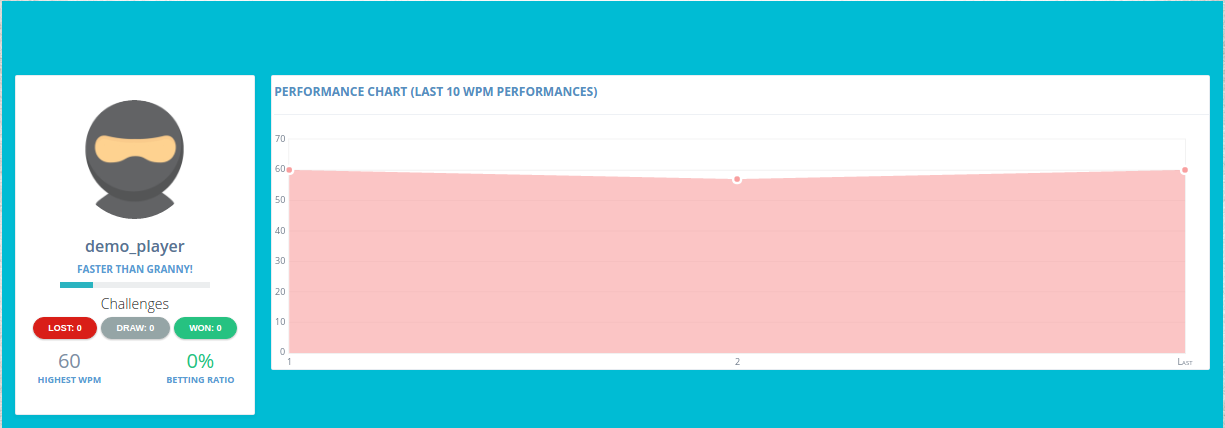
\includegraphics[width=\linewidth]{figures/experiment2/profile.png}
    \caption{Player profile screen}
    \label{fig:game-profile}
\end{figure}

The final element that requires our attention is the concept of game-flow. It was explained in the background section of this chapter that game-flow is the concept of keeping the player constantly engaged while not overwhelming him with problems that are too complex to overcome or too easy that the player gets bored quickly. Our idea of keeping the complexity of the game in the same level as the player's progression and skill improvement in the game is by increasing the total number of words that players have to type within a game-round. The complexity is controlled by the level mechanism of the game. When players progress and reach new levels, they are faced with longer and more complex paragraphs to type. However, one can argue that this is not the best and most optimal way of maintaining game complexity and player's flow zone. Being limited in the amount of resources available to be spent in designing and implementing all the game elements, the proposed idea of defining and maintaining game complexity was the only achievable concept within these constraints. However, ideas to improve the existing design of game complexity will be addressed in the discussion section and as such will be accounted for future work. 
